\documentclass[14pt]{article} %,twocolumn,oneside
% \setlength{\columnsep}{10pt}                    %兩欄模式的間距
% \setlength{\columnseprule}{0pt}                 %兩欄模式間格線粗細

\usepackage{amsthm}                             %定義,例題
\usepackage{amssymb}
\usepackage{fontspec}                           %設定字體
\usepackage{color}
\usepackage[x11names]{xcolor}
\usepackage{listings}                           %顯示code用的
\usepackage{fancyhdr}                           %設定頁首頁尾
\usepackage{graphicx}                           %Graphic
\usepackage{enumerate}
\usepackage{titlesec}
\usepackage{amsmath}
\usepackage[CheckSingle, CJKmath]{xeCJK}
\usepackage{CJKulem}
\usepackage{extsizes}

\usepackage{amsmath, courier, listings, fancyhdr, graphicx}
\topmargin=0pt
\headsep=5pt
\textheight=740pt
\footskip=0pt
\voffset=-50pt
\textwidth=545pt
\marginparsep=0pt
\marginparwidth=0pt
\marginparpush=0pt
\oddsidemargin=0pt
\evensidemargin=0pt
\hoffset=-42pt

%\renewcommand\listfigurename{圖目錄}
%\renewcommand\listtablename{表目錄}

%%%%%%%%%%%%%%%%%%%%%%%%%%%%%

\setmainfont{Consolas}
%\setmonofont{Ubuntu Mono}
\setmonofont{Consolas}
\setCJKmainfont{Noto Sans CJK TC}
\XeTeXlinebreaklocale "zh"                      %中文自動換行
\XeTeXlinebreakskip = 0pt plus 1pt              %設定段落之間的距離
\setcounter{secnumdepth}{3}                     %目錄顯示第三層

%%%%%%%%%%%%%%%%%%%%%%%%%%%%%
\makeatletter
\lst@CCPutMacro\lst@ProcessOther {"2D}{\lst@ttfamily{-{}}{-{}}}
\@empty\z@\@empty
\makeatother
\lstset{                                        % Code顯示
    language=C++,                                   % the language of the code
    basicstyle=\footnotesize\ttfamily,                  % the size of the fonts that are used for the code
    numbers=left,                                  % where to put the line-numbers
    numberstyle=\footnotesize,                  % the size of the fonts that are used for the line-numbers
    stepnumber=1,                                   % the step between two line-numbers. If it's 1, each line  will be numbered
    numbersep=5pt,                                  % how far the line-numbers are from the code
    backgroundcolor=\color{white},              % choose the background color. You must add \usepackage{color}
    showspaces=false,                               % show spaces adding particular underscores
    showstringspaces=false,                     % underline spaces within strings
    showtabs=false,                             % show tabs within strings adding particular underscores
    frame=false,                                        % adds a frame around the code
    tabsize=2,                                      % sets default tabsize to 2 spaces
    captionpos=b,                                   % sets the caption-position to bottom
    breaklines=true,                                % sets automatic line breaking
    breakatwhitespace=false,                        % sets if automatic breaks should only happen at whitespace
    % escapeinside={\%*}{*)},                     % if you want to add a comment within your code
    morekeywords={*},                               % if you want to add more keywords to the set
    keywordstyle=\bfseries\color{Blue1},
    commentstyle=\itshape\color{Red4},
    stringstyle=\itshape\color{Green4},
}


\begin{document}
\pagestyle{fancy}
\fancyfoot{}
%\fancyfoot[R]{\includegraphics[width=20pt]{ironwood.jpg}}
\fancyhead[C]{FJCU}
% \fancyhead[L]{}
% \fancyhead[R]{(\today) \thepage}
\renewcommand{\headrulewidth}{0.4pt}
\renewcommand{\contentsname}{Contents}

\scriptsize
\tableofcontents
\part{語法篇}
\section{基礎資料型態型別}
\subsection{儲存資料}
電腦是以二進位儲存資料,二進位是指數字是由 $0,1$ 組成,相較於常見的十進位是由 $0~9$ 組成,一個 $0$ 或 $1$ 稱為位元 (bit),8 bits 稱為 byte(位元組),byte 是電腦基本儲存單位,下表為各種常見電腦儲存單位。\\
\begin{tabular}{|r|l|} \hline 1B & 1 byte \\\hline 1KB & 1024 bytes \\\hline 1MB & 1024 KBs \\\hline 1GB & 1024 MBs\\\hline \end{tabular}\\
在 C/C++ 裡,將所有的基礎資料型態分成四類說明,依序是整數、浮點數、字元、布林值。
\subsection{整數}
整數分成兩個部分,最左邊的位元表示正負號(0:正,1:負),其餘表示數字。\\
通常會以 int 作為整數型態,int 兼顧範圍大小和記憶體大小。如果存的數字保證不會用到負數的話,可以在前面加上 unsigned,這樣最左邊的位元也會用來表示數字。
\subsubsection{溢位}
上表有給出每種型態的範圍。假設兩個相同型態加總後超過範圍,那麼最高位(最左邊)進位後會被捨去,造成結果和正確值不同,這個狀況稱之為溢位。
\lstinputlisting{Type/overflow.cpp}
% TODO:溢位範例圖
\begin{tabular}{|r|l|l|l|} \hline 名稱 & 別稱 & 位元組 & 範圍 \\\hline short & short int, signed short int & 2 & –32,768 to 32,767 \\\hline unsigned short & unsigned short int & 2 & 0 to 65,535 \\\hline int & signed, signed int & 4 & –2,147,483,648 to 2,147,483,647 \\\hline unsigned int & unsigned & 4 & 0 to 4,294,967,295 \\\hline long long & long long int, signed long long & 8 & –9,223,372,036,854,775,808 to 9,223,372,036,854,775,807 \\\hline unsigned long long & unsigned long long int & 8 & 0 to 18,446,744,073,709,551,615 \\\hline \end{tabular}\\
\subsection{浮點數}
浮點數分成 3 個部分,sign bit(符號):用來表示正負號、exponent(指數):用來表示次方數、mantissa(尾數):用來表示精確度。\\
\begin{figure}
  
\includegraphics[]{Type/IEEE754.png}
  \caption{ASCII from Wiki}
  \label{fig:IEEE754}
\end{figure}\\
\begin{tabular}{|r|l|l|l|l|} \hline 名稱 & 別稱 & 位元組 & 範圍 & 精度 \\\hline float & 無 & 4 & 3.4E +/- 38 & 7 digits \\\hline double & long double & 8 & 	1.7E +/- 308 & 15 digits \\\hline \end{tabular}\\
\subsubsection{浮點數誤差}
浮點數儲存也會有限制,如果小數點後個位數過多,會被捨去造成誤差,float 保證以 10 進位表示時,小數點後 7 位內會是正確,double 則是 15 位。
\lstinputlisting{Type/floatError.cpp}
% TODO:浮點數範例圖
\subsection{字元}
C/C++ 採用 ASCII 字元集,一個數字對應一個字母,但這份字元集只有英文字母、數字、常見的符號,其他國家的文字則無。\\
\begin{tabular}{|r|l|l|l|} \hline 名稱 & 別稱 & 位元組 & 範圍\\\hline char & 無 & 1 & -128 to 127 \\\hline unsigned char & 無 & 1 & 0 to 255 \\\hline wchar & 無 & 2 & 0 to 65,535 \\\hline\end{tabular}\\
\begin{figure}
  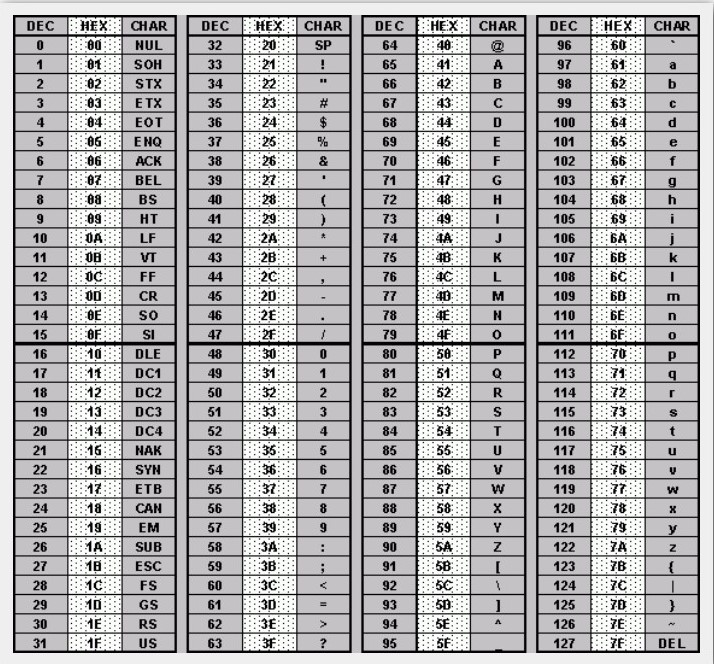
\includegraphics[]{Type/ASCII.jpg}
  \caption{ASCII from http://www.thedawncreative.com/}
  \label{fig:ASCII}
\end{figure}
\subsection{布林值(C++)}
布林值只有兩種植 Ture(1 或是說 非 0)、False(0),當作邏輯變數,相較利用整數型態,有兩個有優勢,一個是節省記憶體,二是可以明確表示是用來記錄 True/False 狀態。\\
\begin{tabular}{|r|l|l|l|} \hline 名稱 & 別稱 & 位元組 & 範圍\\\hline bool & 無 & 1 & 0 to 1 \\\hline\end{tabular}\\
\subsection{後記}
還有一個型態 enum,這裡先不提。\\
\begin{tabular}{|r|l|l|l|} \hline 名稱 & 別稱 & 位元組 & 範圍\\\hline enum & 無 & varies & TBA \\\hline\end{tabular}\\

\section{函式與遞迴}
函式為程式裡的運算單元,可以接受資料,並回傳指定值。main是C/C++程式的入口函式,接受命令列的參數,正常情況會回傳0代表正常運作。\\
以下為其語法
\lstinputlisting{Function/function0.cpp}
範例
\lstinputlisting{Function/function1.cpp}
函式有個特性為自呼叫,也就是自己的區域可以呼叫自己,但要有終止條件,不然會陷入無限遞迴,同時也要避免遞迴過深,造成stack overflow。
\lstinputlisting{Function/function2.cpp}

\subsection{參考}
參考型態代表一個變數的別名,可直接取得變數的位址,並間接透過參考型態別名來操作物件, 作用類似於指標,但卻不必使用指標語法,也就是不必使`*`運算子來提取值。
\lstinputlisting{Function/reference.cpp}
參考型態可用在取代太長的變數(如:`a[x][y][z]`),容易維護。另一個是當函式要傳入可修改的值,可取代指標。
\subsection{傳值}
函式傳入的參數,可以是一般、指標或是參考型態,以下以Swap來介紹
\subsubsection{call by value}
傳入的變數為一般型態,會"複製"一份到函式,原本的變數不會有任何改變。
\lstinputlisting{Function/pass1.cpp}
\subsubsection{call by address/value of pointer}
傳入的變數為指標型態,函式內的變數改變,是對記憶體操作,所以原本的數字也會跟著改變。
\lstinputlisting{Function/pass2.cpp}
\subsubsection{call by reference}
傳入的變數為參考型態,函數內的變數是原本變數的分身,所以函數內變數改變時,原本變數也會跟者改變。
\lstinputlisting{Function/pass3.cpp}

函式有很多用處,一個為模組化,意即相同的部分(最多只差一些參數),寫成一個函式,除了簡潔,在除錯也比較方便。一個是利用自呼叫特性實作遞迴,遞迴可將問題拆解成同類的子問題而解決問題。\\
常見遞迴使用
\begin{enumerate}
\item 分治
\item dp中的top-down
\item 圖/樹的搜索
\end{enumerate}

\section{struct}
struct 可將原本獨立的資料包在一起。例如:三維空間由x座標、y座標、z座標組成。\\
語法:
\begin{enumerate}
\item 型態(type)可以是一般或是指標型態
\item 也可以寫函式或重載運算子
\end{enumerate}
\lstinputlisting{Struct/struct1.cpp}
以下的例子為平面上的點。
\lstinputlisting{Struct/struct2.cpp}
\subsection{建構子(constructor)、解構子(destructor)}
建構子和strcut name同名,是用來初始化struct裡的資料,如果不寫的話,會有預設建構子,裡面的資料都是亂數。根據請況可多載,然而,如果你寫了運算子,一定要寫一個不帶任何參數的運算子,否則的話,像第14行這樣只有宣告,沒加其他東西的的程式碼就不會通過。\\
解構子的名字形式為 $ \sim strcut name$,是在變數離開作用域時運作,不寫的話也是會有預設解構子,在程式比賽中這樣就已足夠。
\subsection{重載運算子}
c++原有的型態都根據需要,定義了各種運算子,但 struct 如果有需要的話,須自己定義。而在競賽中,常需要作排序而需要小於運算子(`<`)。
\section{其他}
\subsection{複雜度}
複雜度是定性描述該演算法執行成本(時間/空間)函式,用來分析資料結構和演算法(DSA)。
\subsubsection{常用函數}
\begin{enumerate}
\item [Big $O$]
用來表示一個複雜度的上界,定義為$f(n)\in O(g(n))\ \ iff\ \ \exists\ c,\ N\in R^{+},\ \forall n \geq  N$ 有 $|f(n)| \leq |cg(n)|$,例如$f(n)=5n^2+4n+1$,我們會注重最高項$5n^2$,且我們會5是常數,得出$f(n)\in O(n^2)$
\item [Big $\Omega$]
用來表示一個複雜度的下界,對於任意的 $f(n) \in O(g(n))$,都有 $g(n) \in \Omega (f(n))$。
\item [Big $\Theta$]
要同時滿足Big $O$和Big $\Omega$
\end{enumerate}
Big $O$ 是我們比較常用的,其他兩個可能再一些地方會用到
    
\subsubsection{常見複雜度}
$O(1) < O(log\ n) < O(n) < O(n\ log\ n) < O(n^2) < O(n^3) < O(2^n) < O(n!)$
另外還有一個在並查集常見,即$O(\alpha(n))$,近似於$O(1)$,可直接當作$O(1)$
\subsubsection{時間/空間複雜度}
時間複雜度,和運算有關,*/\%會比+-還要久,而複雜度得項次會跟迴圈有關,初階競賽只會在意你的項次,只要不要太大基本都會過,進階些比賽,有可能出現常數過大,導致複雜度合理卻還是吃TLE的情況,這時候需要利用"壓常數"技巧,降低時間,讓程式AC。 \\  空間複雜度,則是跟你宣告的變數記憶體總和有關,比時間複雜度容易估計,在樹狀的資料結構,往往需要搭配動態記憶體,才不會因為開太多空間而吃了MLE。 \\  題外話,如果你在你的array不是開在全域內,開了10的5,6次,在執行時跑出RE,那你有以下兩種解決方式
\begin{enumerate}
\item 把array移至全域
\item 加上static,表示靜態變數
\end{enumerate}
\lstinputlisting{Syntax/static.cpp}
指標是紀錄記憶體的位址的變數,不管是基礎型態或自定義型態皆可用指標,指標的可以讓你直接對記憶體操作。而指標對學習者是一到難度高的門檻,但在程式競賽中,是不可或缺的。\\ 指標在程競中會用到的地方是"動態記憶體配置",這在比較進階的資料型態會比較常出現。
\lstinputlisting{Syntax/pointer.cpp}
\lstinputlisting{Syntax/pointer2.cpp}
\subsection{algorithm}
\subsubsection{sort}
這個函式傳入兩個變數,代表容器(array 或是 vector)的頭尾$[a,b)$,這裡的b不會排序,用來指示為結尾,例如要排序a陣列的第0到第5個元素。
\lstinputlisting{Syntax/sort.cpp}
此函數的複雜度圍$O(n\log n)$,n為排序的個數
\subsubsection{min/max}
min和max原本在c定義在math.h內,c++將它移入algorithm中
\lstinputlisting{Syntax/minmax.cpp}
\subsubsection{lower\_bound/upper\_bound}
這兩個函式會在"有序序列"中尋找值,前兩個值放的是容器(array 或是 vector)的頭尾[a,b),第三的是比較的值val。
\lstinputlisting{Syntax/bound1.cpp}
如果要將位置傳換成數字,直接減起始位置就可,下面是一個範例(from cplusplus):
\lstinputlisting{Syntax/bound2.cpp}
\subsubsection{next\_permutation/prev\_permutation}
這兩個函式會幫你的陣列轉為後/前一個字典序,如果沒有後/前一個字典序,這個函式會回傳false,也不會有任何改變,以下為範例(from cplusplus):
\lstinputlisting{Syntax/permutation.cpp}
\subsection{cmath}
\subsubsection{atan/atan2} 
atan/atan2函數是將斜率轉為弧度,如果要在轉為角度就以180度除以PI就好,而atan直接傳入斜率,atan2則是座標,atan2可以處理x=0的狀況,比atan好用。
\lstinputlisting{Syntax/atan.cpp}
\subsubsection{log/log2/log10}
這些都是常用對數函數分別以e,2,10為底
\lstinputlisting{Syntax/log.cpp}
\subsubsection{pow}
此函數會回傳以base為底的exponent次方,若$\geq 10^6$,就會輸出科學記號。
\lstinputlisting{Syntax/pow.cpp}
\subsubsection{sqrt}
此函數會回傳x的根號次方
\lstinputlisting{Syntax/sqrt.cpp}
\subsection{iomanip}
\subsubsection{setw}
這個函式會將傳入的整數設定輸出寬度後輸出。
\lstinputlisting{Syntax/setw.cpp}
\subsubsection{setprecision}
這個函式設定輸出到小數點後幾位。
\lstinputlisting{Syntax/setprecision.cpp}
\subsection{extra syntax}
\subsubsection{break, continue, return}
\begin{enumerate}
\item break:跳出迴圈
\item continue:這輪不做,到下一輪
\item return:跳出函式,並回傳值
\end{enumerate}
在break, continue, return後的else是無用的,因為如果這三種指令執行了,後面的東西就根本不會執行到。
\subsubsection{const}
const用途在於宣告這個變數式不能更動的,這適合用來宣告常數。
\lstinputlisting{Syntax/const.cpp}
\subsubsection{static}
如果一個變數被宣告為static,那麼他只會被宣告一次,直到整個程式結束才被刪除。
\lstinputlisting{Syntax/static2.cpp}
\subsubsection{define}
不知道各位有沒有用過excel中的巨集,他可以幫你做重複性高的動作,C++中的define可以幫你做類似的事。
\lstinputlisting{Syntax/define.cpp}
由上面範例可見,define 可以取代程式中出現的特定字元,還可以帶參數,為了要讓使用define後的結果是正確的,請將取代後的字元括號起來,否則會輸出非預期的結果如上面範例第9行
\lstinputlisting{Syntax/define.cpp}
\subsubsection{typedef}
typedef 可以為型態取別名,在之後用到要宣告該型態的時候,可以打該型態之別名,減省時間。C++11開始可以用using來達到相同的事。
\lstinputlisting{Syntax/typedef.cpp}
\subsubsection{auto}
C++11開始,新增了一個關鍵字叫auto,auto可以自動判別變數型態,但必須給他初始值,否則他無法判別型態,C++14開始,可用在function回傳值
\lstinputlisting{Syntax/auto.cpp}
\subsubsection{range\_based for}
C++11開始有另外一種for是range\_based,他只要給兩個參數,一個變數指定資料型態並提供遍歷,另一個為要遍歷的範圍,例子如下。
\lstinputlisting{Syntax/rangebasefor.cpp}
\subsection{lambda}
方便地定義匿名函式
\subsubsection{lambda-introducer}
也叫Capture clause,宣告外部變數(在可視範圍(scope)內)傳入此函式內的方法。
\begin{enumerate}
\item `[]`:只有兩個中括號,完全不抓取外部的變數。
\item `[=]`:所有的變數都以傳值(call by value)的方式抓取
\item `[\&]`:所有的變數都以傳參考(call by reference)的方式抓取
\item `[x,\&y]`:x變數使用傳值,y變數使用傳參考
\item `[=,\&y]`:除了y變數使用傳參考以外。其餘的變數皆使用傳值的方式
\item `[\&,x]`:除了x變數使用傳值以外,其餘的變數皆使用傳參考的方式
\end{enumerate}
\subsubsection{lambda declarator}
也叫參數清單,傳入此函式對應資料。
\subsubsection{mutable specification}
指定以傳值方式抓取進來的外部變數,如果用不到可省略。
與一般函數的傳入參數之異
\begin{enumerate}
\item 不可指定參數的預設值。
\item 不可使用可變長度的參數列表。
\item 參數列表不可以包含沒有命名的參數。
\end{enumerate}
\subsubsection{例外狀況規格}
指定該函示會丟出的例外,其使用的方法跟一般函數的例外指定方式一樣,如果用不到可省略。
\subsubsection{傳回值型別}
指定lambda expression傳回型別,如果 lambda expression 所定義的函數很單純,只有包含一個傳回陳述式(statement)或是根本沒有傳回值的話,可省略(optional)
\subsubsection{compound-statement}
亦稱為 Lambda 主體(lambda body),跟一般的函數內容一樣。\\ \\
最後來看個lambda範例,結束這一章節。
\lstinputlisting{Syntax/lambda1.cpp}
\lstinputlisting{Syntax/lambda2.cpp}
\part{資料結構}
\section{基礎資料結構}
\subsection{什麼是STL?}
標準函式庫(Standard Template Libiary),C++內建的資料結構。
\subsection{型態模板}
當你要使用容器時,你必須要告訴C++說,你的資料型態是什麼,型態模板的用途就是在於此。\\
用法:$C <T> name$\\
而容器內部東西不會只有一個,像map就需要兩種型態。\\
$map <T1, T2> name$\\
有時候參數不須寫滿,不寫滿的地方的值為預設值。
\subsection{迭代器}
如果你想在容器中遍歷,你可能想用下標運算子`[]`,但不是所有容器都像陣列,都有支援下標運算子,所以C++為每個容器都提供一個資料型態叫"迭代器",你可以把迭代器當成一種指標,假設有一個迭代器it,加上星號`*`可以存取IT所指向的內容,依據迭代器的強到弱可分為三種:
\begin{enumerate}
\item 隨機存取(Random Access):可與整數做+-法、遞增及遞減
\item 雙向(Bidirectional)迭代器:遞增及遞減
\item 單向(Forward)迭代器:只能遞增
\end{enumerate}
根據用法可分為兩種:
\begin{enumerate}
\item 輸入(Input)迭代器:讀取迭代器指向的內容,,所有的迭代器都可以當作輸入迭代器。
\item 輸出(Output)迭代器:更改迭代器指向的內容時,除了常數(const)迭代器(也就是規定不能更動迭代器指向的內容)以外,所有的迭代器都可以當作輸出迭代器。
\end{enumerate}
C++在許多容器中提供正向和逆向迭代器,前者由前往後,後著由後往前,宣告時分別為$C::iterator$及$ C::reverse\_iterator$,每種迭代器分別有一對迭代器代表頭尾,如下表,注意end系列指向該容器最後一項的後一項,不要對他做人和取值或修改。\\ \\
\begin{tabular}{|l|c|c|}
	\hline &正向&逆向 \\
	\hline 可改值&C.begin()\ C.end()&C.rbegin()\ C.rend()\\
	\hline 不可改值&C.cbegin()\ C.cend()&C.crbegin()\ C.crend()\\
    \hline
\end{tabular}
\subsection{stack 堆疊}
有兩個端口,其中一個封閉,另一個端口負責插入、刪除的資料結構
\lstinputlisting{BasicDS/stack.cpp}
\begin{enumerate}
\item 標頭檔:<stack>
\item 建構式:stack <T> s
\item s.push(T a):插入頂端元素,複雜度$O(1)$
\item s.pop():刪除頂端元素,複雜度$O(1)$
\item s.top():回傳頂端元素,複雜度$O(1)$
\item s.size():回傳元素個數,複雜度$O(1)$
\item s.empty():回傳是否為空,複雜度$O(1)$
\end{enumerate}
\lstinputlisting{BasicDS/stack2.cpp}
\subsection{queue 佇列} 
有兩個端口,一個負責插入,另一個端口負責刪除的資料結構
\lstinputlisting{BasicDS/queue.cpp}
\begin{enumerate}
\item 標頭檔:<queue>
\item 建構式:queue <T> q
\item q.push(T a):插入尾端元素,複雜度$O(1)$
\item q.pop():刪除頂端元素,複雜度$O(1)$
\item q.front():回傳頂端元素,複雜度$O(1)$
\item q.size():回傳元素個數,複雜度$O(1)$
\item q.empty():回傳是否為空,複雜度$O(1)$
\end{enumerate}
\lstinputlisting{BasicDS/queue2.cpp}
\subsection{deque 雙向佇列} 
有兩個端口,皆負責刪除、插入的資料結構
\begin{enumerate}
\item 標頭檔:<deque>
\item 建構式:deque <T> dq
\item dq.push\_front(T a),dq.push\_back(T a):插入頂端/尾端元素,複雜度$O(1)$
\item dq.pop\_front(),dq.pop\_back():刪除頂端/尾端元素,複雜度$O(1)$
\item dq.front(),dq.back():回傳頂端/尾端元素,複雜度$O(1)$
\item dq.size():回傳元素個數,複雜度$O(1)$
\item dq.empty():回傳是否為空,複雜度$O(1)$
\end{enumerate}
\subsection{list}
陣列如果要從中間插入一個元素,需要將其後面所有元素搬移一格,需耗費$O(n)$,連結串列(linklist)能只花$O(1)$完成插入。
\lstinputlisting{BasicDS/linklist1.cpp}
\lstinputlisting{BasicDS/linklist2.cpp}
但有時候我們也可以利用idnex取代指標來實作linklist,兩種做法各有自己的優缺點。\\
C++提供list函式庫實作雙向串列
\begin{enumerate}
\item 標頭檔:`<list>`
\item 建構式:`list <T> L`
\item L.size():回傳元素個數,複雜度$O(1)$
\item L.empty():回傳是否為空,複雜度$O(1)$
\item L.push\_front(T a),L.push\_back(T a):插入頂端/尾端元素,複雜度$O(1)$
\item L.pop\_front(),L.pop\_back():刪除頂端/尾端元素,複雜度$O(1)$
\item L.insert(iterator it,size\_type n,T a):在 it 指的那項的前面插入 n 個 a 並回傳指向 a 的迭代器。複雜度 $O(n)$。
\item L.erase(iterator first,iterator last):把 $[first,last)$ 指到的東西全部刪掉,回傳 last。複雜度與砍掉的數量呈線性關係,如果沒有指定 last,那會自動視為只刪除 first 那項。
\item L.splice(iterator it,list\& x,iterator first,iterator last):first 和 last 是 x 的迭代器。此函式會把 $[first,last)$ 指到的東西從 x 中剪下並加到 it 所指的那項的前面。x 會因為這項函式而改變。若未指定 last,那只會將 first 所指的東西移到 it 前方。複雜度與轉移個數呈線性關係。
\end{enumerate}
\lstinputlisting{BasicDS/list.cpp}
\subsection{array}
更安全方便的陣列
\begin{enumerate}
\item 標頭檔:<array>
\item 建構式:array <T,N> a
\item a.size():回傳元素個數,複雜度$O(1)$
\item a.fill(T val):將每個元素皆設為val,複雜度$O(size)$
\end{enumerate}
\lstinputlisting{BasicDS/array.cpp}
\subsection{vector}
動態陣列,可改變長度
\begin{enumerate}
\item 標頭檔:<vector>
\item 建構式:vector <T> v
\item v[i]:回傳v的第i個元素,複雜度$O(1)$
\item v.push\_back(T a):插入尾端元素,複雜度$O(1)$
\item v.size():回傳元素個數,複雜度$O(1)$
\item v.resize():重設長度,複雜度$O(1)$
\item v.clear():清除元素,複雜度$O(size)$
\item 兩特化
    \begin{enumerate}
    \item vector<char>:string
    \item vector<bool>:bitset
    \end{enumerate}
\end{enumerate}
\lstinputlisting{BasicDS/vector.cpp}
\subsection{string} 
可變動長度的字元陣列
\begin{enumerate}
\item 標頭檔:<string>
\item 建構式:string s
\item s=t:讓s的內容和t一樣,複雜度通常是$O(size(s)+size(t))$
\item s+=t:將t加到s後面,複雜度通常是$O(size(s)+size(t))$
\item s.cstr():回傳和s一樣的C式字串,複雜度$O(1)$
\item cin>>s:輸入字串至s,直到讀到不可見字元
\item cout<<s:輸出字串s
\item getline(cin,s,char c):輸入s直到遇到字元c,未指定c時,c為預設字元。
\end{enumerate}
\lstinputlisting{BasicDS/string.cpp}
\subsection{bitset} 
節省的bool陣列,可當二進位位元運算
\begin{enumerate}
\item 標頭檔:<bitset>
\item 建構式:bitset <N> b(a)
\item b[a]:存取第 a 位,複雜度 $O(1)$。
\item b.set():將所有位元設成1。複雜度 $O(N)$。
\item b.reset():將所有位元設成 0。複雜度 $O(N)$。
\item b(位元運算):不管是一元、二元運算皆可。二元位元運算長度需一致。複雜度 $O(N)$。
\item b.count():回傳 b 有幾個位元是 1。複雜度 $O(N)$。
\item b.flip():將所有位元的 0、1 互換。複雜度 $O(N)$。
\item b.to\_string():回傳一個字串和 b 的內容一樣。複雜度 $O(N)$。
\item b.to\_ulong():回傳一個 unsigned long 和 b 的內容一樣 (在沒有溢位的範圍內)。複雜度,$O(N)$。
\item b.to\_ullong():回傳一個 unsigned long long 和 b 的內容一樣 (在沒有溢位的範圍內),複雜度 $O(N)$。
\end{enumerate}
\subsection{priorty\_queue 優先佇列} 
維護最大/小值,可插入、刪除、及詢問最大/小值,一種實作為binary heap
\lstinputlisting{BasicDS/heap.cpp}
\begin{enumerate}
\item 標頭檔:<queue>
\item 建構式:priorty\_queue <T> pq
\item 建構式:priorty\_queue <T,Con,Cmp> pq
\item 建構式:priorty\_queue <T,Con,Cmp> pq(iterator first, iterator seecond)插入$[first,second)$內的東西
\item pq.push(T a):插入元素a,複雜度$O(\log size)$
\item pq.pop():刪除頂端元素,複雜度$O(\log size)$
\item pq.top():回傳頂端元素,複雜度$O(1)$
\item pq.size():回傳元素個數,複雜度$O(1)$
\item pq.empty():回傳是否為空,複雜度$O(1)$
\end{enumerate}
\lstinputlisting{BasicDS/PQ.cpp}
\subsection{pair} 
兩個資料型態組織合盟
\begin{enumerate}
\item 標頭檔:`<utility>`
\item 建構式:`pair <T1,T2> p`
\item p.first,p.second:p的第一、二個值
\item make\_pair(T1 a1,T2 a2):回傳一個(a1,a2)的pair
\end{enumerate}
\subsection{tuple} 
generalize的pair
\begin{enumerate}
\item 標頭檔:`<tuple>`
\item 建構式:tuple<T1,T2...> t
\item `get<i>(t)`:回傳 t 的第 i 個值。
\item make\_tuple(T1 a1,T2 a2,...):回傳一個 (a1,a2,...)的tuple。
\end{enumerate}
\subsection{set/map 自查找平衡二元樹}
set和map支援插入、刪除及查詢一個值,不同的是,set會回傳鍵值,map則是回傳對應值,也可以說set的鍵值和對應值一樣
\subsection{set} 
\begin{enumerate}
\item 標頭檔:`<set>`
\item 建構式:`set <T1> s`
\item s.size():回傳元素個數,複雜度$O(1)$
\item s.empty():回傳是否為空,複雜度$O(1)$
\item s.clear():清除元素,複雜度$O(size)$
\item s.insert(T1 a):加入元素 a,複雜度 $O(\log size)$。
\item s.erase(iterator first,iterator last):刪除 $[first,last)$,若沒有指定 last 則只刪除 first,複雜度$O(\log size)$與加上元素個數有關係。
\item s.erase(T1 a):刪除鍵值 a,複雜度 $O(\log size)$。
\item s.find(T1 a):回傳指向鍵值 a 的迭代器,若不存在則回傳 s.end(),複雜度 $O(\log size)$。
\item s.lower\_bound(T1 a):回傳指向第一個鍵值大於等於 a 的迭代器。複雜度 $O(\log size)$。
\item s.upper\_bound(T1 a):回傳指向第一個鍵值大於 a 的迭代器。複雜度 $O(\log size)$。
\end{enumerate}
\lstinputlisting{BasicDS/set.cpp}
\subsection{map}
\begin{enumerate}
\item 標頭檔:`<map>`
\item 建構式:`map <T1, T2> m`
\item m.size(),m.empty(),m.clear(),m.erase(iterator first,iterator last),m.erase(T1 a),m.find(T1 a),m.lower\_bound(T1 a),m.upper\_bound(T1 a):同 set。
\item `m[a]`:存取鍵值 a 對應的值,若 a 沒有對應的值,會插入一個元素,使 a 對應到預設值並回傳之。複雜度 $O(\log size)$。
\item m.insert(pair<T1,T2> a):若沒有鍵值為 a.first 的值,插入一個鍵值為 a.first 的值對應到a.second,並回傳一個 pair,first 是指向剛插入的元素的迭代器、second 是 true;若已經有了,回傳一個 pair,first 是指向鍵值為 k.first 的元素的迭代器,second 是 false。複雜度 $O(\log size)$。
\lstinputlisting{BasicDS/map.cpp}
\end{enumerate}
\subsubsection{multi-系列}
可插入重複元素代價為map無法用下標運算子
\begin{enumerate}
\item equal\_range(T1 a):回傳iterator的pair<lower\_bound(a),upper\_bound(a)>,為a所在範圍
\item erase(T1 a):刪除所有元素a,如果只要刪除一個,用s.erase(s.find(a))
\end{enumerate}
\subsubsection{unorder\_系列}
降低常數,期望複雜度少一個 log,代價為不會排序,沒有lower\_bound/upper\_bound,也不會依鍵值大小遍歷。迭代器為單向。
\subsection{題目}
\subsubsection{stack,queue,deque}
先來看一題題目\\ \\
(zjd555)
在平面上如果有兩個點 (x,y) 與 (a,b),我們說 (x,y) 支配(Dominate)了(a,b)這就是指 x $\geq$ a
而且 y $\geq$ b;用圖來看就是 (a,b) 座落在以 (x,y) 為右上角的一點無的區域中。\\ 
對於平面上的任意一個有限點集合而言,一定存在有若干個點,它們不會被集合中的內一點所支配,這些個數就構成一個所謂的極大集合。請寫一個程式,讀入一個新的集合,找出這個集合中的極大值。\\
簡單的說  若找不到一點在 (x,y) 的右上方,則 (x,y) 就要輸出\\ \\
我們能肯定最右上角的點一定是極大點,再來的極大點一定都在他的右下方,那我們就以座標排序,先以y座標由大到小排序,再以x座標由大到小排序,每找到一個極大點,就找下一個y值比它小,x比它到的點,那也是極大點,就這樣以此類推。\\
我們觀察到極大集合中,如果先以Y值排序由大到小排序,X值會由小到大,如果我們發現,答案的候選人,有如果...就大於/小於...的關係,我們就稱答案有"單調性"。單調性這個東西筆者覺得很玄,我沒辦法明確定義什麼事單調性,需要多多寫題目才能自己感覺出來。\\
下列提供stack,queue,deque的題目,前半部分是基礎應用,後半部分是關於單調性的。
\begin{enumerate}
\item UVa514(Stack 應用)
\item UVa673(Stack 應用)
\item ZeroJudge d016(Stack 後續運算法)
\item UVa10935(Queue 應用)
\item UVa12100(Queue 應用)
\item Uva246(Deque 應用)
\item UVa11871(stack 單調)
\item TIOJ1618(Deque 單調)
\end{enumerate}
\subsubsection{list}
\begin{enumerate}
\item ZeroJudge d718
\item TIOJ 1225
\item TIOJ 1930
\end{enumerate}
\subsubsection{string}
\begin{enumerate}
\item ZeroJudge a011(getline 應用)
\item Zerojudge d098(StringStream 應用,請自行查詢)
\end{enumerate}
\subsubsection{PriortyQueue}
\begin{enumerate}
\item Uva 10954
\item Uva 1203
\end{enumerate}
\subsubsection{set,map}
\begin{enumerate}
\item ZeroJudge d512(Set 應用)
\item UVa 10815(Set 應用)
\item Zerojudge d518(Map 應用)
\item UVa 484(Map 應用)
\end{enumerate}










\section{演算法}
\subsection{何謂演算法}
簡言之就是解決問題的方法,用程式語言把他明確地列出。
\subsection{枚舉}
枚舉是最直觀的演算法,將有可能的答案都搜過一遍,當然沒有頭緒的搜尋可能會得到龐大的複雜度,要根據題目的性質來降低複雜度。
\subsubsection{回朔}
枚舉有時能用遞迴實作,在遇到不可能的情形馬上回傳,這種方法就叫做回朔ㄊ。
\subsubsection{特殊枚舉方式}
\begin{enumerate}
\item [二進位] 利用二進位來表示集合內有哪些元素要用,進而枚舉所有元素子集,但受限於時間複雜度$O(2^n)$,集合的元素個數通常只有30個(甚至15個)。   
\item [字典序] 利用 next\_permutation 或 prev\_permutation 達到枚舉元素的先後順序。時間複雜度為$O(N!)$
\end{enumerate}
% \subsubsection{爬行法}
\subsubsection{折半枚舉}
有時遇到複雜度$O(2^n)$的算法,在無法用其他方法降低複雜度,可以試著將元素切成兩半,降低n,再用其他算法組合起來。
\subsubsection{題目}
\begin{enumerate}
\item UVa 11059(區間列舉)
\item UVa 1481(區間列舉)
\item UVa 10976(減少列舉範圍)
\item UVa 750(回朔)
\item UVa 524(回朔)
\item UVa 11464
\item UVa 1326(折半枚舉)
\end{enumerate}
\subsection{貪心}
對於一個問題,始終使用同一種方法,採取在目前狀態下最好或最佳(即最有利)的選擇。\\
有的貪心很直觀,有的就需要通靈才解得出來,往往做題目一開始想到的辦法是錯的,直到做到一半才發現。所以我們需要證明方法是不是對的,這往往需要時間練習,才不會到比賽遇到時,花了很多時間去解題。\\
\subsubsection{證明的辦法}
\begin{enumerate}
\item 試圖構造出反例,發現他不存在。
\item 如果存在更佳解的答案比你做出來的還好,那這組解一定可以再做得更好,進而達到反證出更佳解不存在。
\item 使用遞迴證法:(1) 證明基底是對的。(2) 假設小問題是好的。(3) 你一定可以用最好的方法來將問題簡化成剛才假設是好的小問題。
\end{enumerate}
\subsubsection{題目}
\begin{enumerate}
\item UVa 11729
\item UVa 11292
\item UVa 11389
\item UVa 1445
\item UVa 993
\item TIOJ 1441
\end{enumerate}
\subsection{二分搜}
對於一個函數$F(n)$,如果存在一個x,對於所有 $\geq x$ 的a,$F(a)=$ true,反之$F(a)=$ false,基於這樣的單調性,就可以用二分搜。
\lstinputlisting{BasicA/binarySearch.cpp}
有些題目為"最多/最少為何會成立",那麼如果你可以在良好的時間檢查出"如果代價是 x,那可不可以達成目標",並且x具有單調性,那麼你可以轉換成"如果代價是 x,那可不可以達成目標"傳換成$F(x)$,對答案(x)進行二分搜。\\
二分搜要注意兩件事,一個是無限迴圈,要避免它可以在腦中先模擬一下。一個是在實數中二分搜,因為實數的稠密性,題目會有誤差容忍(例如$10^{-6}$),只要在誤差內都是容許的。
\subsubsection{三分搜}
對於U型函數(例如$y=F(x)=x^2$),我們想要找尋其極值,意謂其左右兩側皆各自遞增/遞減,我們可以利用三分搜來解決(二分搜只能解決全體單調性,不能解決有兩邊的)。\\
考慮三分後從左到右四個採樣點的關係
\begin{enumerate}
\item $S(a) < S(b) < S(c) < S(d)$,此時最小值一定不在最右邊
\item $S(a) > S(b) < S(c) < S(d)$,此時最小值一定不在最右邊
\item $S(a) > S(b) > S(c) < S(d)$,此時最小值一定不在最左邊
\item $S(a) > S(b) > S(c) > S(d)$,此時最小值一定不在最左邊
\end{enumerate}
這段描敘還可以再簡化
\begin{enumerate}
\item $S(b) < S(c)$,此時最小值一定不在最右邊
\item $S(b) > S(c)$,此時最小值一定不在最左邊
\end{enumerate}
每次都至少可以讓區間縮小$\frac{1}{3}$
\lstinputlisting{BasicA/3Search.cpp}
\subsubsection{題目}
\begin{enumerate}
\item Uva 714
\item Uva 1421
\item Uva 11627
\item neoj 72(三分搜)
\end{enumerate}
\subsection{分治}
分治法會把問題分解成子問題(分),解決完再合併回原本的問題(治)。\\
分治分成以下步驟
\begin{enumerate}
\item 切割:把一個問題切成子問題然後遞迴
\item 碰底:碰到不能再切割或是明顯有答案(也許無解),就算出答案再回傳
\item 合併:利用傳回來的子問題算出答案然後回傳
\end{enumerate}
\subsubsection{合併排序法}
一個利用分治實作的排序法,之後逆序數對也會利用他的概念來實作。
\begin{enumerate}
\item 切割:把序列分成兩半然後遞迴
\item 碰底:直到序列長度為1,這時候已為一個排好的序列,直接回傳
\item 合併:利用傳回來的兩串序列進行排序
\end{enumerate}
\subsubsection{更多的經典題目}
\begin{enumerate}
\item 快速排序法。
\item 逆序數對。(經典問題,搭配 Merge Sort)
\end{enumerate}
\subsubsection{題目}
\begin{enumerate}
\item uva 1608
\item uva 10810
\item uva 11129
\item uva 10245
\end{enumerate}

\section{DP}
\subsection{特性}
\begin{enumerate}
\item 重複子問題:相同的一個子問題,需要多次查詢。
\item 最佳子結構:當問題被拆成若干個規模較小的問題時,可以透過這些子問題得到這個問題的最佳解。
\item 無後效性:子問題不會互相呼叫,一定存在一個能完整求值的計算順序。
\end{enumerate}
\subsection{步驟}
DP通常會被定義成一個算出答案的函數,函數的參數個數可變,對於一種題目可能有不同種的定義辦法,要看自己如何決定。
\begin{enumerate}
\item 訂出狀態
\item 導出轉移:從一個子問題的答案推到另一個
\item 設好基底:有些問題明顯有答案(也許無解),就直接算出答案
而時間複雜度,通常就會是「使用到的狀態個數」乘上「轉移時間」了。
\end{enumerate}
\subsection{費式數列}
費式數列是個看到膩的數列,我們就把他的DP式列出來
\begin{enumerate}
\item 狀態:$f(x)$代表費式數列第$n$項
\item 轉移:$f(n)=f(n-1)+f(n-2)$
\item 基底:$f(n)=n,where$ $n\leq 1$
\end{enumerate}
我們先用遞迴的方式寫寫看
\lstinputlisting{DP/fib01.cpp}
原因是因為他有很多重複的子問題,那麼我們就以"空間換時間"的辦法來加速。
\lstinputlisting{DP/fib02.cpp}
這種用遞迴實作的叫做Top-down,好處是容易寫出來,缺點是遞迴的常數非常大。\\
而費式數列還有一種用迴圈的寫法。
\lstinputlisting{DP/fib03.cpp}
這種的迴圈實作的叫做Buttom-up,雖然比較難寫,但是時間常數比遞迴小,有時可以利用"滾動陣列"來壓縮空間。\\
第一個單純遞迴的版本,其複雜度等同費式數列第N項。第二、三版本,每項費式數列只會被算一次,所以複雜度為$O(N)$。
\subsection{滾動陣列}
如果一個DP式只會用到臨近的項數,就可以捨棄其他用不到的,藉此壓縮空間。
例如:費式數列只會用到前兩項,我們就用取餘數來實作滾動陣列,注意被餘數要保持正數。
\lstinputlisting{DP/fib04.cpp}
\subsection{題目}
\begin{enumerate}
\item UVa10003(區間DP)
\item UVa10285
\item zerojudge d212
\item UVa11310
\end{enumerate}
接下來我們談論一些經典問體
\subsection{背包問題}
背包問題中,會給你背包的容量C,以及N樣物品,它們有不同的重量w和價值v,背包裡物品價值總和最大為何?
\subsubsection{0/1背包}
01背包限制每樣物品最多只能放一個。那就來寫DP式。
\begin{enumerate}
\item 狀態:$dp[n][i]$ $=$ 使用 $1 ∼ n$ 個物品湊出重量 i 時,所可得到的最大價值。
\item 轉移:$dp[n][i] = max(dp[n − 1][i − w[n]] + v[n], dp[n − 1][i])$
\item 基底:$dp[0][0] = 0$, $dp[0][i] = −INF$ when $i>0$
\end{enumerate}
以防在DP的過程不小心用到,湊不出來的狀態要設成負無限大,或是使用if判斷取代預設。
\lstinputlisting{DP/01backpack1.cpp}
現在時間空間複雜度皆為$O(NC)$,而空間可以在持續優化。\\
記得剛剛說過的滾動陣列嗎?先回去看看DP式,$dp[n]$轉移只會用到$dp[n-1]$,所以我們只要保留前一行(行列的區分我不管)就好了。
\lstinputlisting{DP/01backpack2.cpp}
這樣的空間複雜度為$2N$,再來,我們發現第二個維度,他只會用到小於它的地方,那麼我們可以只用一行。但是要由後往前轉移,這樣才不會讓還沒轉移到的狀態,取到已轉移的,保證該項物品只會被取一次。
\lstinputlisting{DP/01backpack3.cpp}
\subsubsection{無限背包}
無限背包每樣物品能放無限多個。同樣要先列出DP式。
\begin{enumerate}
\item 狀態:$dp[n][i]$ $=$ 使用 $1 ∼ n$ 個物品湊出重量 i 時,所可得到的最大價值。
\item 轉移:$dp[n][i] = max(dp[n − 1][i − w[n]] + v[n], dp[n][i − w[n]] + v[n], dp[n − 1][i])$
\item 基底:$dp[0][0] = 0, dp[0][i] = −INF$ when $i>0$
\end{enumerate}
如果第i個物品重量為$w_i$,那麼最多可以放$\frac{C}{w_i}$次,要多一層迴圈來模擬。
\lstinputlisting{DP/infbackpack1.cpp}
時間複雜度為$O(NC\Sigma\frac{C}{w_i})$\\
我們現在回到之前01背包最後一個範例,當初要由後往前,是為了保證每個物品都只放了一個,而現在我們要放越多越好,那我們就由前面開始轉移就行了。
\lstinputlisting{DP/infbackpack2.cpp}
時間複雜度為$O(NC)$
\subsubsection{有限背包}
有限背包每樣物品能放限制最多可以放$a_i$。這裡請讀者自己列出DP式。
我們一樣由01背包延伸,一樣物品最多可以放$a_i$個,那麼迴圈最多要跑$a_i$次,這樣整體時間複雜度為$O(NC\Sigma a_i)$。\\
有限背包又沒有像無限背包那麼好的性質,但如果我們帶入二進位的觀念,第$i$位代表$2^{i-1}$,我們把$a_i$個物品拆成$1,2,4...,2^k$次方個枚舉,那麼我們可以將時間複雜度降為$O(NC\Sigma(\log a_i))$
講道更進階一點的DP,會學到"單調堆列優化",能將時間複雜度降為$O(NC)$
\subsection{題目}
\begin{enumerate}
\item zerojudge b184(01背包)
\item UVa10664(01背包)
\item UVa10898(無限背包)
\item Uva10086(有限背包)
\item TIOJ 1387(有限背包)
\end{enumerate}
\subsection{最長共同子序列 (Longest Common Subsequence)}
子序列是指一個序列去除某些元素後所形成的新序列(當然也可以不刪除任何東西),而所謂的最長共同子序列,則是要求兩個字串去除元素後變成相同的序列,最長可以為何。這題觀念是簡單的,在這裡就列出dp式供讀者自行解讀。
\begin{enumerate}
\item 狀態:$dp[i][j]$ $=$ 使用 $a[1]~a[i]$和$b[1]~b[j]$ 的LCS長度。
\item 轉移:$dp[i][j] =\left\{ \begin{array}{cc}
dp[i-1][j-1]+1 & if\ a[i]=b[j]\\
max(dp[i-1][j],dp[i][j-1]) & else
\end{array} \right\}$
\item 基底:$dp[i][0]=dp[0][i]=0$ when $i \geq 0$
\end{enumerate}
\subsection{題目}
\subsection{最長遞增子序列 (Longest Increasing Subsequence)}
給你一個序列長度為N,求最長遞增子序列的長度。\\
你可能會在其他地方看見一維DP式,在這裡不提,有興趣可以去演算法筆記看,這裡要介紹另一種DP式
\begin{enumerate}
\item 狀態:$dp[n][i]$ $=$ 使用 $1 ∼ n$ 個數字湊出長度 $i$ 的 LIS,末端數字最小為何。
\item 轉移:$dp[n][i] =\left\{ \begin{array}{cc}
min(dp[n-1][i],a[n]) & if\ a[n]>dp[n-1][i-1]\\
dp[n-1][i] & else
\end{array} \right\}$
\item 基底:$dp[i][0] = INF, dp[0][j] = −INF$ when $i \geq 0$ and $j \geq 1$
\end{enumerate}
時間複雜度為$O(n^2)$。\\
再來,我們令$g[i]=dp[x][i]$, where $1\leq x \leq N$,我們會發現$g[i]$為一個嚴格遞減序列,而且改的數字剛好的$a[i]$,更妙的是,被改的數字為$lower_bound(a[i])$,我們就可以用二分搜來得到$O(n\log n)$的演算法了。
\lstinputlisting{DP/LIS.cpp}
\subsection{題目}
\begin{enumerate}
\item Uva10405(LCS)
\item UVa11456(LIS)
\item UVa11790(LIS)
\end{enumerate}
\section{Graph}
圖是由邊集合和點集合所形成的圖形,這種圖形通常用來描述某些事物之間的某種特定關係。頂點用於代表事物,連接兩頂點的邊則用於表示兩個事物間具有這種關係。\\
數學式為$G=(V,E)$。$G$代表圖(Graph),$V$代表點(vertex),$E$代表邊(edge)。
\subsection{術語}
在深入圖論中,我們先介紹一些術語,這些術語在後面的內容,不時會扮演著關鍵角色。
\begin{enumerate}
\item 無向邊、有向邊:邊具有方向性,無向邊代表邊沒有指定方向,$(u,v)$和$(v,u)$等價;有向邊則有指定方向,$(u,v)$和$(v,u)$是不同的。
\item 無向圖、有向圖、混合圖:無向圖是只有無向邊的圖,類似地,有向圖是只有有向邊的圖,混和圖則是包含無向邊和有向邊。
\item 點、邊個數:一般來說會用$|V|$、$|E|$來表示,在表示複雜度時,為了方便會用$V$、$E$來表示
\item 權重(weight):在點或邊上附帶一個數字稱做"權重",邊上權重較常見,權重通常代表代價,例如所需花費時間或金錢。
\item 相鄰 (adjacent):無向圖中,兩個點 $u$, $v$ 相鄰代表存在一個邊 $e_i = (u, v)$。
\item 指向 (consecutive):有向圖中, $u$ 指向 $v$ 代表存在一個邊 $e_i = (u, v)$。
\item 度(degree):無向圖中,一個點連到的邊數稱為"度",在有向圖稱為出度(out-degree,簡稱 $d_{out}$)及入度(in-degree,簡稱 $d_{in}$),分別代表該點指向別點及被指向的邊數。
\item walk:一條由$x$到$y$的路徑$x=v_1,v_2,v_3...,v_k=y$。
\item trail:一條不重複邊的walk。
\item 迴路(circut):起點和終點一樣的trail。
\item path:一條不重複點(起點和終點例外)的walk。
\item 環(cycle):起點和終點一樣的path。
\item 自環 (loop):一條邊 $e_i = (u, v)$ 滿足 $u = v$,$e_i$ 即稱為自環。
\item 重邊 (multiple edge):在一張圖中,存在 $e_i$, $e_j$ 滿足 $i$ != $j$ and $e_i = e_j$,則稱為重邊。
\item 連通 (connected):無向圖中,若 $u$ 和 $v$ 存在路徑,則 $u$ 和 $v$ 連通。若一群點兩兩連通,則這些點都連通。
\end{enumerate}
\subsection{儲存}
至於圖要怎麼存起來呢,以下介紹兩種辦法。設$V$為點數,$E$為邊數。
\subsubsection{相鄰矩陣(adjacency matrix)}:開一個 $V \times V$ 的資料結構$M$(通常會用二維陣列),$M[a][b]$代表的是點$a$至$b$的邊數或權重。空間複雜度$O(V^2)$。加、刪邊時間複雜度 $O(1)$。
\subsubsection{相鄰串列(adjacency list)}:開$V$個可變長度的資料結構 (通常在 C++ 用 vector、在C用 linked list),第$i$個裡面放所有第$i$個點指向的點的編號 (和邊權或其他邊的資訊)。空間複雜度$O(V + E)$,加邊時間複雜度$O(1)$、刪邊時間複雜度$O(V)$。
至於使用時機,如果邊數較密,且頻繁地需要找尋兩點之間的權重,那麼相鄰矩陣比較適合,其餘情況則是用相鄰串列。
\subsection{遍歷}
存好圖後,為了獲得某些資訊,需要一些讀取的方法,這些方法我們叫做"遍歷"。以下介紹兩種方法:DFS和BFS。
\subsubsection{DFS}
找到一條新的路就繼續找下去,直到沒有新的路時,原地返回。通常用遞迴實作或用stack維護。
\lstinputlisting{Graph/DFS.cpp}
\subsubsection{BFS}
\lstinputlisting{Graph/BFS.cpp}
把所有看到的路都加入清單中,並且以加入的順序來遍歷。通常以queue來維護。\\
BFS和DFS的時間複雜度皆為$O(V+E)$,空間複雜度皆為$O(V)$。\\
注意,圖不一定完全連通,我們通常會另外開一個陣列(bitset)紀錄是否拜訪過。
\subsubsection{題目}
\begin{enumerate}
\item zerojudge a290(給你一張有向圖,問你可不可以由A走到B)
\item zerojudge a982(二維迷宮問題)
\item zerojudge a634(馬步問題)
\item UVa 572
\end{enumerate}
\subsection{樹}
樹是一種特殊的圖,有許多算法都是由樹發展出來。
\subsubsection{特性}
以下這些無向圖的敘述都是在表示樹,這些敘述在競賽中有時能引導出答案。
\begin{enumerate}
\item 為連通圖且$|V|=|E|+1$
\item 任意兩個點之間存在唯一路徑
\item 為連通圖,但拔掉一條邊即為不連通(分成兩張連通圖)。
\item 沒有環,但加上一條邊會形成環。
\item 若節點編號存在順序,除了第一個節點,每個節點都會伸出一條邊連到順序比自己前面的節點。
\end{enumerate}
\subsubsection{術語}
樹同樣也有一些術語要知道的。
\begin{enumerate}
\item 根(root):樹的一個代表性的點,通常會被當遍歷的起點,有給定根點的樹叫"有根樹"。至於無根樹依照題目需求,有時要隨機找一個點當根。
\item 葉解點(leaf):度數為1的節點,有根樹的根結點則會是題目需求來決定是否為葉節點。
\item 父節點、子節點:有根樹中,兩個相連的節點,比較接近樹根的為父節點,反之為子節點。
\item 祖先(ancestor)、子孫(descandent):有根樹中,節點到根結點中,所有的節點皆為祖先。反過來說,該節點是他的祖先的子孫。依題目所需,有時自己也是自己的祖先(尤其是根最常這樣定義)。
\item 距離(distance):為兩個點所形成路徑之邊數,或是路徑上權重之和。
\item 深度(depth):有根樹中,節點到根結點之距離。
\item 高度(height):有根樹中,節點到與它距離最大的葉節點的距離稱為高度。根的高度稱為這整顆樹的高度。
\item 子樹(subtree):設有兩棵樹$T$,$T_1$,如果$V_1\in V$,$E_1\in E$,那麼我們說 $T_1$ 為 $T$ 的子樹
\item N元樹:每個節點最多有N個節點,稱為N元樹。
\end{enumerate}
\subsection{二元樹}
二元樹在程式競賽中常常被討論,有許多資料結構都是二元樹,例如STL提到的heap。
\subsubsection{遍歷}
基於根結點遍歷順序,二元樹的遍歷有"前序、中序、後序"三種辦法,通常DFS會使用前序來實作,如果想要得到任何一種順序的結果,只要改變輸出的順序。
\subsubsection{二元搜尋樹(Binary Search Tree, BST)}
二元搜尋樹是二元樹的應用,利用遞迴方式來定義,如下:
\begin{enumerate}
\item 根結點的值大於左子節點的值,小於右子節點的值。
\item 其左右子樹亦為二元搜尋樹。
\end{enumerate}
用上敘定義,就可以建造出BST,不過如果我們將一個以排序的串列建成BST,會發現BST會"退化"成一條傾斜的串列。BST本身不實用,重要在於它的推廣結構,例如AVL樹、紅黑樹、treap,不過這些資料結構比較進階,在這裡先不提。
\subsection{並查集}
並查集是一種樹狀結構,他支援兩件事
\begin{enumerate}
\item 查詢所隸屬集合
\item 合併兩個集合
\end{enumerate}
我們把集合轉化成樹,一顆樹代表一個集合,樹根代表集合的老大,查詢隸屬集合就回傳樹根是誰(一個樹餔可能有兩顆樹根吧),合併的時侯,就把一顆樹的樹根只到另一顆,以下為詳細的描述。
\subsubsection{初始}
一開始的時候,每個點自成一個集合,所以把樹根都設為自己。
\subsubsection{查詢}
查詢的時候,要查到樹根為自己的點,為止否則的話就要繼續查。
\subsubsection{狀態壓縮}
在合併之後原本被指向的樹根就沒用了,我們可以一邊做查詢時,一邊做更新。
\subsubsection{啟發式合併}
建立一個$h[i]$代表樹的高度,亦是元素最大遞迴次數,$h[i]$一開始為1。再來,我們每次都讓高度小的高度大的合併,如果遇到高度一樣的,就讓合併別人的樹高度加1。如果要把高度變為x,則至少需要$2^x$個點,由此推出N個點所形成最高之高度為$\log(N)$。\\
\lstinputlisting{Graph/DisjointSet.cpp}
複雜度為$O(\alpha(N))$。並查集最常用的地方是最小生成樹的Kruskal’s algorithm。
\subsubsection{題目}
\begin{enumerate}
\item zerojudge d808
\item UVa 1160
\item UVa 10158(陣列開兩倍)
\item UVa 1329(帶權並查集)
\end{enumerate}
\subsection{最小生成樹(Minimun Spanning Tree, MST)}
在一張圖中,如果有子圖剛好維也為一顆樹,我們就稱該子圖為生成樹。現在我們在圖上加上權重,而在所有的生成樹中,權重最小的,我們稱為"最小生成樹",最小生成樹並不唯一,以下介紹幾種最小生成樹的演算法。
\subsubsection{Kruskal’s algorithm}
Kruskal’s algorithm的概念是,合併兩顆MST的時候,加入連接兩顆樹中,最小權重的邊。所以我們就利用greedy,將邊依權重由小到大排序,如果邊的兩邊是在不同的MST,我們就把合併(並查集應用於此),反之就跳過。排序需花$O(E\log E)$的時間,選邊需要花$O(E\alpha(V))$的時間,總共時間複雜度$O(E(\log E+\alpha(V)))$
\lstinputlisting{Graph/Kruskal.cpp}
\subsubsection{Prim’s algorithm}
Prim’s algorithm的思維則是,將一棵MST連出的邊中,加入權重最小的邊(距離最近的點),重複執行後得出最小的生成樹。在實作上,首先取一個點當MST,更新所有與它相鄰的點,更新後把距離最小的點加入MST(不用並查集),持續執行更新及加入點的動作,直到所有點都已加入MST。維護最小距離用priority\_queue維護,每個點只會被合併一次,每條邊都只會遍歷一次,複雜度$O((V+E)logE)$。另外有一個資料結構用費波那契堆(fibonacci heap)可以達到 $O(E+V\log V)$。但是因為它常數比較大,實作複雜,我們不會使用它。總體而言,Kruskal比Prim好用。
\subsubsection{Borůvka’s algorithm}
Borůvka’s algorithm和Prim一樣都在加入MST和最鄰近的點,不一樣的是,它讓所有的MST一起做這件事。每次找出每棵MST外權重最小的邊,並加入MST(如果權重一樣,就找索引值最小的),檢查是否只剩一棵MST,如果不是就重複掃描的動作,這裡一樣用並查集維護聯通性。\\
最差的情況為每次都剛好兩兩成對合併,這樣最多只會執行$\log V$次,整題複雜度為$O((V+E)\log V)$,f)。期望複雜度可以達到$O((V+E))$ (因為每次並查集都會被合併+查詢,所以$\alpha$可以完全省略)。
\subsubsection{題目}
\begin{enumerate}
\item zerojudge a129
\end{enumerate}
\subsection{最短路徑}
\subsubsection{術語}
\begin{enumerate}
\item 負邊:權重為負的邊
\item 負環:權重和為負的環
\item 點源:成為起點的點,分成單源頭及多源頭。
\item 鬆弛:單源頭最短路徑中,對於任意兩個點$u,v$,起點$s$到它們的距離$d_u,d_v$,如果$d_u>d_v+w_{u,v}$,$w_{u,v}$為邊$(u,v)$的權重,我們可以讓$d_u$更新為$d_v+w_{u,v}$,讓$s$到$u$的距離縮短,這個動作稱為"鬆弛"。 
\end{enumerate}
\subsubsection{Floyd-Warshall Algorithm}
為多源頭最短路徑,求出所有點對的最短路徑。\\
Floyd-Warshall是動態規劃,以下是他的dp式。
\begin{enumerate}
\item 狀態:$dp[k][i][j]$ 代表,若只以點 $1 ∼ k$ 當中繼點的話,則 $dp[k][i][j]$ 為 $i$ 到 $j$ 的最短路徑長。
\item 轉移:$dp[k][i][j] = min(dp[k − 1][i][k] + dp[k − 1][k][j], dp[k − 1][i][j])$
\item 基底:$dp[0][i][j] = \left\{ \begin{array}{cc}
w[i][j] & if\ w[i][j]\ exists\\
INF & else
\end{array} \right\}$
\end{enumerate}
時/空間複雜度皆為$O(V^3)$,然而此DP是可以滾動,所以空間複雜度可降為$O(V^2)$\\
\lstinputlisting{Graph/FW.cpp}
執行的時候如果$dp[i][j]<0$,代表存在負環,Floyd-Warshall是可以判斷負環。
\subsubsection{單點源最短路徑}
求出一個點到所有點的最短路徑,其實就是以起點為根,最短路徑是由父節點鬆弛而來的最短路徑樹。我們找最短路徑,就是一直把鬆弛,直到所有點都不能鬆弛,所有點都獲得最短路徑了。要蓋出最短路徑樹,就只要把點指向最後一次被誰鬆弛就好了。
\subsubsection{Bellman-Ford Algorithm}
為單點源最短路徑,設起點的最短路徑為0,其他點為無限大,每次枚舉所有邊枚舉,因為最短路徑不會經過同樣的邊第二次,所以只要執行$V-1$輪,複雜度為$O(VE)$。如果執行第V次時還有邊可以鬆弛,代表有負環,Bellman-Ford也可以當成負環的判斷方法。\\
\lstinputlisting{Graph/bellmanford.cpp}
此演算法還有一個優化版本叫做Shortest Path Faster Algorithm(SPFA),他的做法是枚舉起點是鬆弛過的邊,以鬆弛過的點除非被重新鬆弛,否則不會更動。預期複雜度為$O(V+E)$,不過最差狀況仍為$O(VE)$。
\subsubsection{Dijkstra’s Algorithm}
同樣為單點源最短路徑,他的想法和Prim's Algorithm類似,每次把離樹根最近的點加入最短路徑樹裡,並把所有與該點相連的邊鬆弛,已經加入的點不會在被鬆弛。使用priority\_queue的複雜度為$(V+E)\log E$,使用費波那契堆,複雜度為s$O(E+V\log V)$
\lstinputlisting{Graph/dijkstra.cpp}
\subsubsection{題目}
\begin{enumerate}
\item UVa 534
\item UVa 10048
\item UVa 929(方格上)
\item UVa 11090
\end{enumerate}

\section{數論}
數論是數學中,專門在研究整數性質的領域,涉及質數、組合等,被譽為最純的數學領域,是數學的皇后。
\subsection{質數}
質數為因數只有1和自己的數,質數問題在程式競賽中常常遇到,通會建立質數表來查詢質數。
\subsubsection{一般篩法}
每找到一個質數x,就知道2x, 3x, 4x...都不是質數,把他們從候選名單剃除。
\lstinputlisting{Math/PrimeTable1.cpp}
複雜度可到$O(N\log\log N)$,如果不從平方開始剃除,則會退化至$O(N\log N)$
\subsubsection{線性篩法}
將一般篩法優化至$O(N)$,我們期望每個合數都只被其最小質因數剔除,這樣可以確保其均攤的線性。實作上,我們讓每一個數去替除"自己乘上$<=$其質因數的所有質數"的數字即可。
\lstinputlisting{Math/PrimeTable2.cpp}
\subsection{因數}
我們能將任意一個正整數做質因數分解,形式為$N=P_{1}^{x_{1}}P_{2}^{x_{2}}P_{3}^{x_{3}}...=\Pi P_{i}^{x_{i}}$,根據此形式,我們可以求出任一正整數的因數個數及因數總和
\begin{enumerate}
\item [因數個數] $(x_{1}+1)(x_{2}+1)(x_{3}+1)...=\Pi (x_{i}+1)$
\item [因數總和] $(P_{1}^{0}+P_{1}^{1}+...+P_{1}^{x_{1}})(P_{2}^{0}+P_{2}^{1}+...+P_{2}^{x_{2}})...=\Pi\Sigma_{j=0}^{x_{i}}(P_{i}^{j})$
\end{enumerate}
\subsection{最大公因數和最小公倍數}
最大公因數(Greatest Common Divisor, GCD),可以用輾轉相除法求得。
\lstinputlisting{Math/GCD.cpp}
複雜度為$O(\log(min(a,b)))$,最慘狀況發生在兩數為費式數列相鄰項時,C++<algorithm>有內建的\_\_gcd可以用。\\
最小公倍數(Least Common Multiple,LCM),則為兩數相乘再除以他們的GCD,為避免溢位狀況,可先將一數除以GCD,再乘以另外一數。
\subsubsection{題目}
\begin{enumerate}
\item zerojudge a007(質因數分解)
\item TIOJ 1040 (連分數)
\end{enumerate}
\subsection{模}
\subsubsection{性質}
\begin{enumerate}
\item [加法] $(a+b)\ \%\ p= (a\ \%\ p +b\ \%\ p )\ \%\ p$
\item [減法] $(a-b)\ \%\ p= (a\ \%\ p -b\ \%\ p +p)\ \%\ p$
\item [乘法] $(a*b)\ \%\ p= (a\ \%\ p *b\ \%\ p )\ \%\ p$
\item [次方] $(a^b)\ \%\ p= ((a\ \%\ p )^b)\ \%\ p$
\item [加法結合律] $((a+b)\ \%\ p+c)\ \%\ p = (a+(b+c))\ \%\ p$
\item [乘法結合律] $((a*b)\ \%\ p*c)\ \%\ p = (a*(b*c))\ \%\ p$
\item [加法交換律] $(a+b)\ \%\ p=(b+a)\ \%\ p$
\item [乘法交換律] $(a*b)\ \%\ p=(b*a)\ \%\ p$
\item [結合律] $((a+b)\ \%\ p*c)= ((a*c)\ \%\ p +(b*c)\ \%\ p )\ \%\ p$
\end{enumerate}
如果$a\equiv b (\mod m)$,我們會說$a,b$在模$m$下同餘,關於同餘也有一些性質。\\
參考文章:https://wangwilly.github.io/willywangkaa/2018/05/08/Discrete-mathematics-Chinese-Remainder-Theorem/
\begin{enumerate}
\item [整除性] $a\equiv b \quad (\mod m) \Rightarrow c \cdot m  = a - b , c \in \mathbb{Z}$\\ $\Rightarrow a \equiv b\quad ( \mod m ) \Rightarrow m \; | \; a-b$
\item [遞移性] 若 $a \equiv b \quad (\mod c) , b \equiv d \quad (\mod c)$\\ 則 $a \equiv d (\mod c)$
\item [保持基本運算] $\left \{ \begin{matrix} a \equiv b (\mod m)\\ c \equiv d (\mod m)\end{matrix}\right. \Rightarrow \left\{\begin{matrix}a \pm c \equiv b \pm d (\mod m)\\ a \cdot c \equiv b \cdot d (\mod m)\end{matrix}\right.$
\item [放大縮小模數] 令$k \in \mathbb{Z}^+ , a \equiv b \quad (\mod m) \Leftrightarrow k \cdot a \equiv k \cdot b \quad (\mod k \cdot m)$
\end{enumerate}
\subsubsection{快速冪}
我們常常遇到求$a^b mod\ c$為多少的題目,最簡單的作法是用迴圈花b次算出答案,但是在b很大時就無法快速算出。這時如果拆成$a^1,a^2,a^4,...,a^{2^x}$,先分別計算在乘起來,這樣只要花費$O(\log b)$的時間即可。
\lstinputlisting{Math/abc.cpp}
\subsubsection{模逆元}
模逆元是取模下的反元素,即為找到$a^{-1}$使得$aa^{-1}\equiv\ 1\ mod\ c$。如果a要在mod c下有反元素,那麼$gcd(a,c)=1$,根據貝祖定理,可知存在整數$x,y$,使得$ax+cy=gcd(a,c)=1$,這裡的$x$即為a的反元素,我們可以修改找GCD的辦法,找出$a$的反元素。
\lstinputlisting{Math/extgcd.cpp}
\subsubsection{題目}
\begin{enumerate}
\item TIOJ 1199
\item zerojudge b430
\item zerojudge a289(求模逆元)
\end{enumerate}
\subsection{一些定理}
\subsubsection{歐拉函數}
歐拉函數計算對於一個整數N,小於等於N的正整數中,有幾個和N互質。通常用$\Phi(n)$表示。其公式為$\Phi(N)=N\times\Pi_{p|N}(1-\frac{1}{p})$\\
\lstinputlisting{Math/Phi.cpp}
歐拉函數還有一些性質\\
如果 p 是質數:$\Phi(p) = p-1$以及$\Phi(p^k)=p^{k−1}\times (p−1)$\\
如果 pq 互質:$\Phi(pq) = \Phi(p)\times\Phi(q)$\\
根據這些性質,我們能寫出一個類似質數篩法的作法。
\lstinputlisting{Math/PhiTable.cpp}
\subsubsection{費馬小定理}
給定一個質數$p$及一個整數$a$,那麼:\\
$a^p \equiv a (\mod p)$\\
如果$gcd(a,p)=1$,則:\\
$a^{p-1} \equiv 1 (\mod p)$\\
\subsubsection{歐拉定理}
歐拉定理是比較generate版本的費馬小定理。給定兩個整數n和a,如果$gcd(a,n)=1$,則\\
$a^{\Phi(n)} \equiv 1 (\mod n)$\\
如果n是質數,$\Phi(n)=n-1$,也就是費馬小定理。
\subsubsection{Wilson's theorem}
給定一個質數$p$,則:\\
$(p-1)!\equiv -1 (\mod p)$
\subsubsection{題目}
\begin{enumerate}
\item UVa 12493(歐拉定理)
\item UVa 1434(Wilson's theorem)
\end{enumerate}
\subsection{中國剩餘定理}
中國剩餘定理,又稱中國餘數定理,是數論中的一個關於一元線性同餘方程組的定理。用來解決像下面這種問題:\\
"有物不知其數,三三數之剩二,五五數之剩三,七七數之剩二。問物幾何?",這題答案為$23+105n,n>=0$\\
列出這種問題的式子(設$m_i$兩兩互質):
$\left \{ \begin{matrix} X\equiv a_1 (mod\ m_1)\\ X\equiv a_2 (mod\ m_2)\\ \cdot \\ \cdot \\ X\equiv a_n (mod\ m_n)\end{matrix}\right.$\\
解決這類問題最簡單適用枚舉來求解,不過如果範圍太大就會吃TLE了。因此我們 ,我們設$M=\Pi_{i=1}^{n} m_i$,令$x_1\ mod\ m_1\equiv a_1$,而對其他$m_i$皆整除,拆解$x_1$成為$x_1=(M/m_1)r_1$亦即$(M/m_1)r_1\equiv a_1 (mod\ m_1)$,用找模逆元的方式求出$x_1$。$x_2,x_3,...,x_n$也是依照這個辦法求出,最後$X=(\Sigma_{i=1}^{n} x_i)\ mod\ M\ +\ kM\ (k>=0)$。\\
總共有n個式子,每個式子都要找一次模逆元,所以複雜度為$O(n \log m)$
\subsubsection{題目}
\begin{enumerate}
\item zerojudge c641
\end{enumerate}
\section{參考}
\begin{enumerate}
\item 建中講義
\item 板中講義
\item 資訊之芽
\item cplusplus
\item cppreference
\item openhome
\item https://blog.gtwang.org/programming/lambda-expression-in-c11/
\end{enumerate}

\end{document}